\chapter{Clase 3. Tangram circular y problemas}
\textbf{13/02/2025}
\section{Tangram circular}

Los materiales y herramientas necesarias para el tangram circular fueron:
    \begin{itemize}
        
        \item Rectangulo de fomi
        \item Regla
        \item Compás
        \item Lápiz
        
    \end{itemize}

Elaboración:
    \begin{enumerate}
        
        \item Coloca la hoja en horizontal y traza $l_1$ de forma vertical de modo que divida el fomi en dos partes y una de ellas sea de $\frac{2}{3}$ del tamaño total del largo
        \item Traza $l_2 \perp l_1$ dividiéndola en dos mitades
        \item Con el compás, traza $C(O,r)$ donde $O = l_1 \cap l_2$
        \item Sean $A,B \in l_1$ en lados opuestos de $l_2$ tal que  estos puntos son las intersecciones de $C(O,r)$ con $l_1$ y análogamente para $C,D \in l_2$ (Sea $C$ elemento del lado de $l_1$ de mayor longitud)
        
         \item Traza los segmentos $\overleftrightarrow{AC}$ y $\overleftrightarrow{BC}$
         \item Abre el compás al tamaño del diámetro y traza dos arcos de circunferencia iniciando el trazo desde el punto $A$ y el segundo en $B$ de modo que ambos interseccten $l_2$ en el lado de $l_1$ que contiene a C
         \item Sea $E$ la intersección de $\overleftrightarrow{AC}$ con el arco de circunferencia que pasa por $A$. análogamente para $F$
         \item Traza una circunferencia $C'(C,r'')$ donde $r'' = CF $

         \item Traza otra circunferencia $C'(D,r'')$ y sean $G,H$ los puntos de intersección de $C'(D,r'')$ con $l_1$
         \item Traza los segmentos $\overline{DG}$ $\overline{DH}$
      \end{enumerate}

Las figuras trazadas deben quedar como la siguiente imagen
\begin{center}
   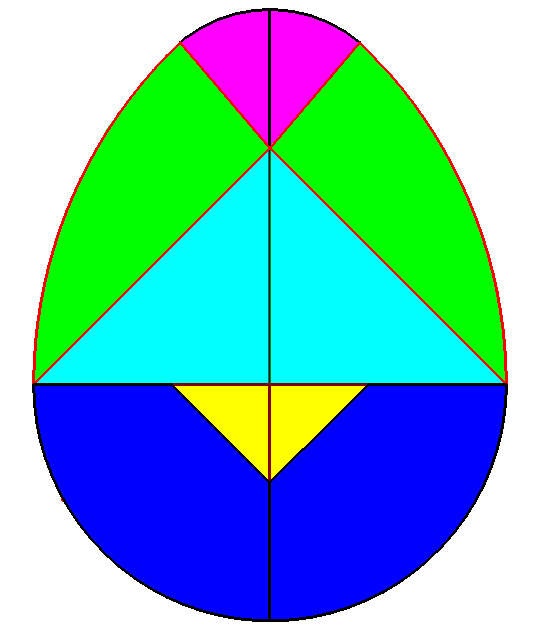
\includegraphics[scale=0.05]{clase3/huevodecolon.jpg}
\end{center}

Despues de realizar el tangram, se debían hacer ciertas figuras que mostró la maestra en clase, de las cuales una se hizo en clase y la otra quedó de tarea.

\begin{center}
   \begin{tabular}{ccc}
      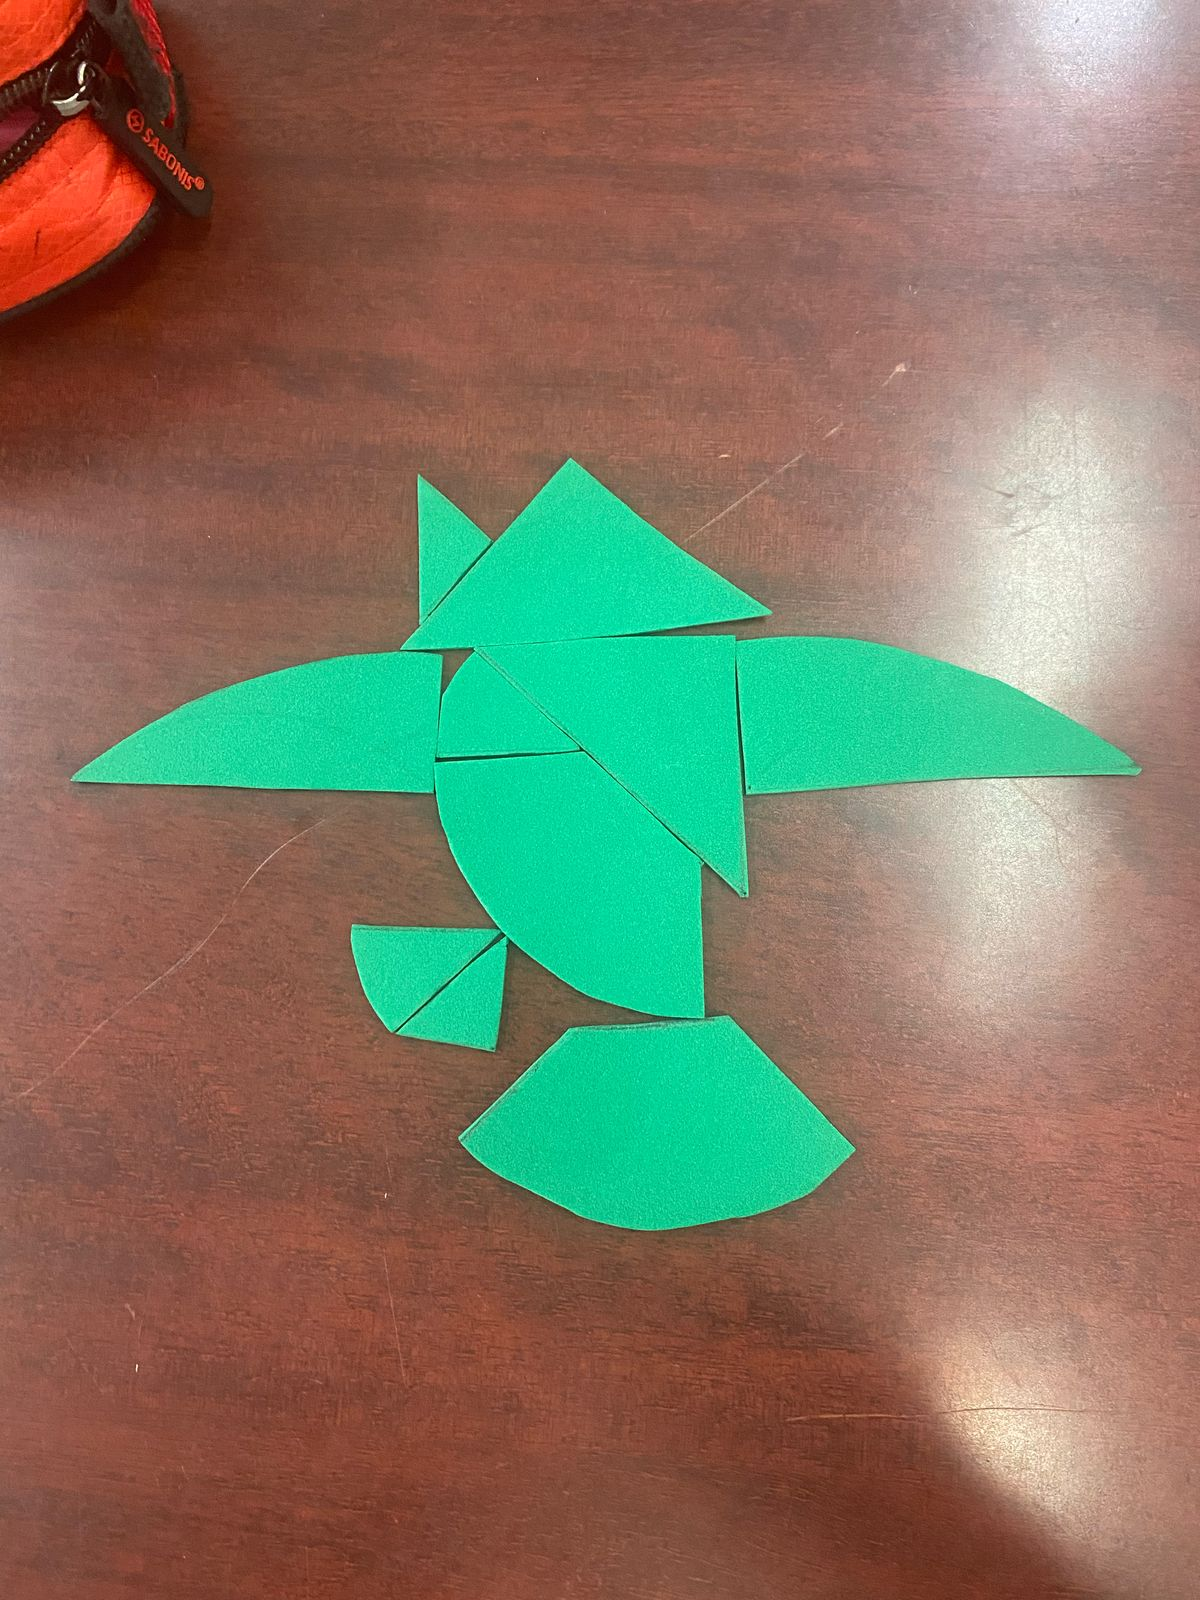
\includegraphics[scale=0.09]{clase3/Pajaro.jpeg}&&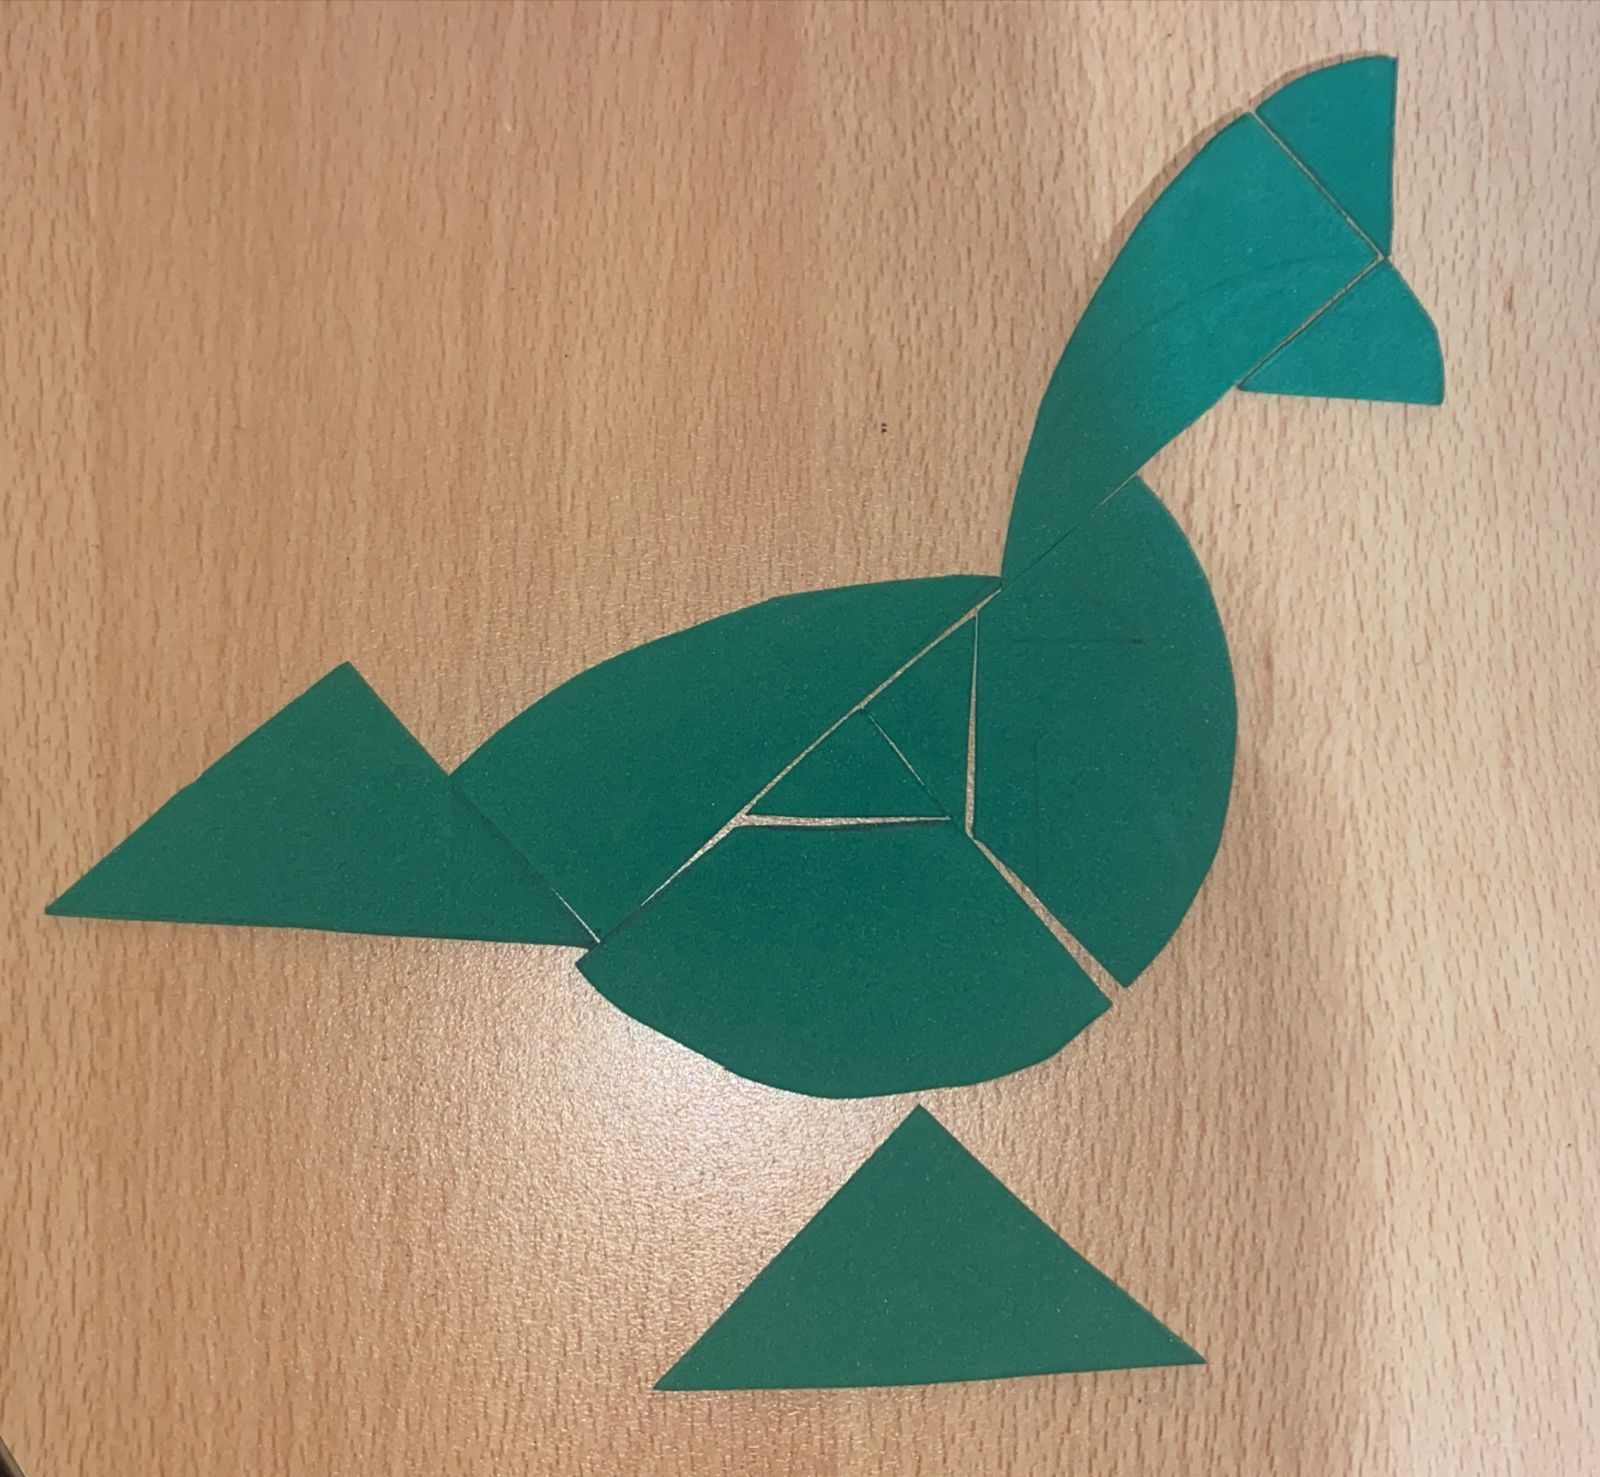
\includegraphics[scale=0.09]{clase3/Pajaro2.jpeg}
   \end{tabular}
\end{center}

La manera en como resolví el problema fue analizando cada borde de mis piezas de tangram contra los bordes de las figuras a realizar, acomodando primero las piezas que parecían más faciles por estar a simple vista sin necesidad de unirles más piezas.

\section{Acertijos}\label{sec:C3ACERTIJOS}

\begin{ejem}\label{ejem:c3P1}
   Un campesino lleva al mercado para vender un lobo, una cabra y un repollo; al marchar así con su mercancía debe poner cuidado en que el lobo no ataque a la cabra y que la cabra no se coma el repollo.
   Se encuentra con un río que le conviene cruzar de esta manera: como no puede ni debe hacer pasar al mismo tiempo más de una cosa que con-duce, ha de poner cuidado en que el lobo en ausencia del campesino no pueda atacar a la cabra ni la cabra comerse el repollo, puesto que si él no está siempre presente la cabra comerá el repollo o será comida por el lobo. Cabe preguntarse entonces cómo podría hacer pasar sus mercaderías al otro lado del río sin sufrir ningún daño
\end{ejem}
   \textbf{SOLUCION.}Primero el campesino debe de cruzar a la cabra, después la deja del otro lado regresa y se lleva ya sea el lobo o el repollo, (en este caso tomaremos al repollo) cuando llega al mismo lado de la cabra, deja el repollo y en su regreso lleva consigo a la cabra y al momento de llegar con el lobo, deja la cabra en el lado inicial,  y se lleva al lobo para dejarlo al mismo lado que el repollo y al momento de regresar nuevamente cruza a la cabra. Así, el campesino habrá cruzado a los tres, sin que la cabra o el repollo sean comidos.

\begin{ejem}\label{ejem:c3P2}
   Un herrero debe formar una cadena con 15 eslabones y tiene a la mano 5 trozos de cadena con 3 eslabones cada uno. ¿Cuál es la cantidad mínima de eslabones que debe romper y soldar? Para lograr su objetivo.
\end{ejem}
   \textbf{SOLUCIÓN.}El herrero rompe 4 trozos de eslabones por alguno de los extremos de ellos y los solda al otro conjunto de eslabones en el extremo en el cual no fue roto ninguno

\begin{ejem}\label{ejem:c3P3}
   Tienes 9 monedas aparentemente idénticas, pero una de ellas es falsa y pesa más que las demás. Dispones de una balanza de dos platillos y puedes realizar solo dos pesajes para identificar cuál es la moneda falsa. ¿Cómo puedes determinar cuál es la moneda falsa bajo las condiciones pedidas?
\end{ejem}
   \textbf{SOLUCIÓN.}Primero se hacen tres grupos de tres monedas cada uno. Luego se toman dos grupos al azar y se pesan a partir de aquí tenemos dos casos:
   \begin{enumerate}
      \item La balanza se mantiene equilibrada.
      \item La balanza no se mantiene equilibrada
   \end{enumerate}
   En el caso uno podemos deducir que la moneda falsa está en el tercer grupo que no fue pesado y y de este mismo grupo se toman dos monedas y nuevamente hay dos casos, el primero en donde ambas monedas están equilibradas, esto nos indica que la moneda falsa es aquella que no fue pesada, y el segundo caso es aquel en donde una moneda pesa más que la otra.
   Para el segundo caso en donde la balanza no se mantuvo equilibrada, se toma el grupo que pesó más y la moneda falsa se halla de manera análoga al primer caso.

\begin{ejem}\label{ejem:c3P4}
   Un hombre vende vino pero sólo dispone de una medida de tres litros. Llega al negocio otro hombre que lleva una medida de cinco litros y que pide al tabernero cuatro litros de vino; la cuestión es saber cómo podrá el tabernero dar al cliente esos cuatro litros puesto que solo tiene un jarro de tres litros en tanto que el jarro del cliente es de cinco litros.
\end{ejem}
   \textbf{SOLUCIÓN.}Primero llenas la medida de 3l ,luego la vacías en la medida de cinco y nuevamente hasta que se llenen los 5l,  pues en la medida de tres quedará uno. Después de esto se desecha el vino de la medida de 5l y el litro de la jarra de tres se vierte en la medida más grande se vuelve a llenar la jarra de 3 l y se vacía en la de cinco obteniendo así, los 4l

\begin{ejem}\label{ejem:c3P5}
   Las monedas en la foto forman la punta de una flecha que apunta hacia arriba. Cambia de posición tres de ellas para obtener una punta de flecha que apunta hacia abajo.
   \begin{center}
      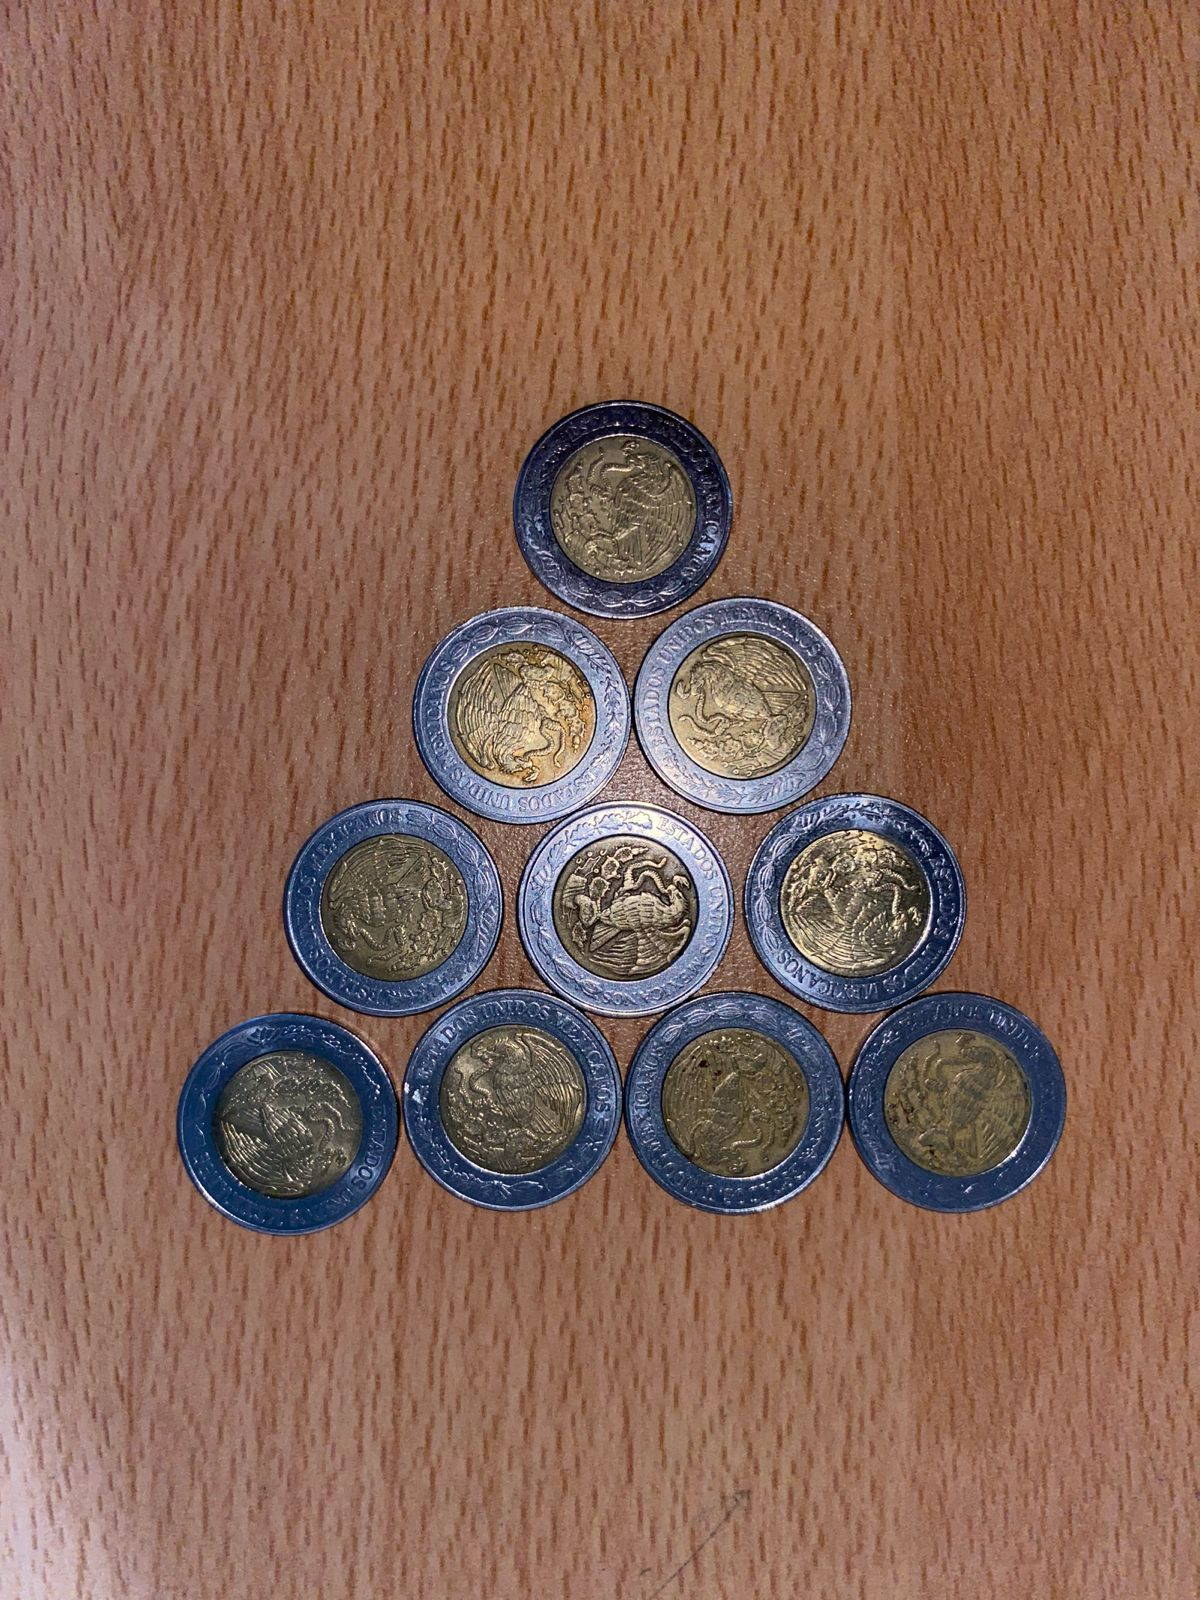
\includegraphics[scale=0.09]{clase3/Flecha.jpeg}
   \end{center}
\end{ejem}
   \textbf{SOLUCIÓN 1.} Primero enumeramos cada fila de monedas, según la cantidad. Después de esto, observamos que la base debía tener cuatro monedas, por lo cual tomamos dos monedas de la fila cuatro, y las pasamos a la fila dos y la moneda de la fila, uno la pasamos debajo de la fila cuatro.
   \\
   \begin{center}
      
      \begin{tabular}{c c c}
            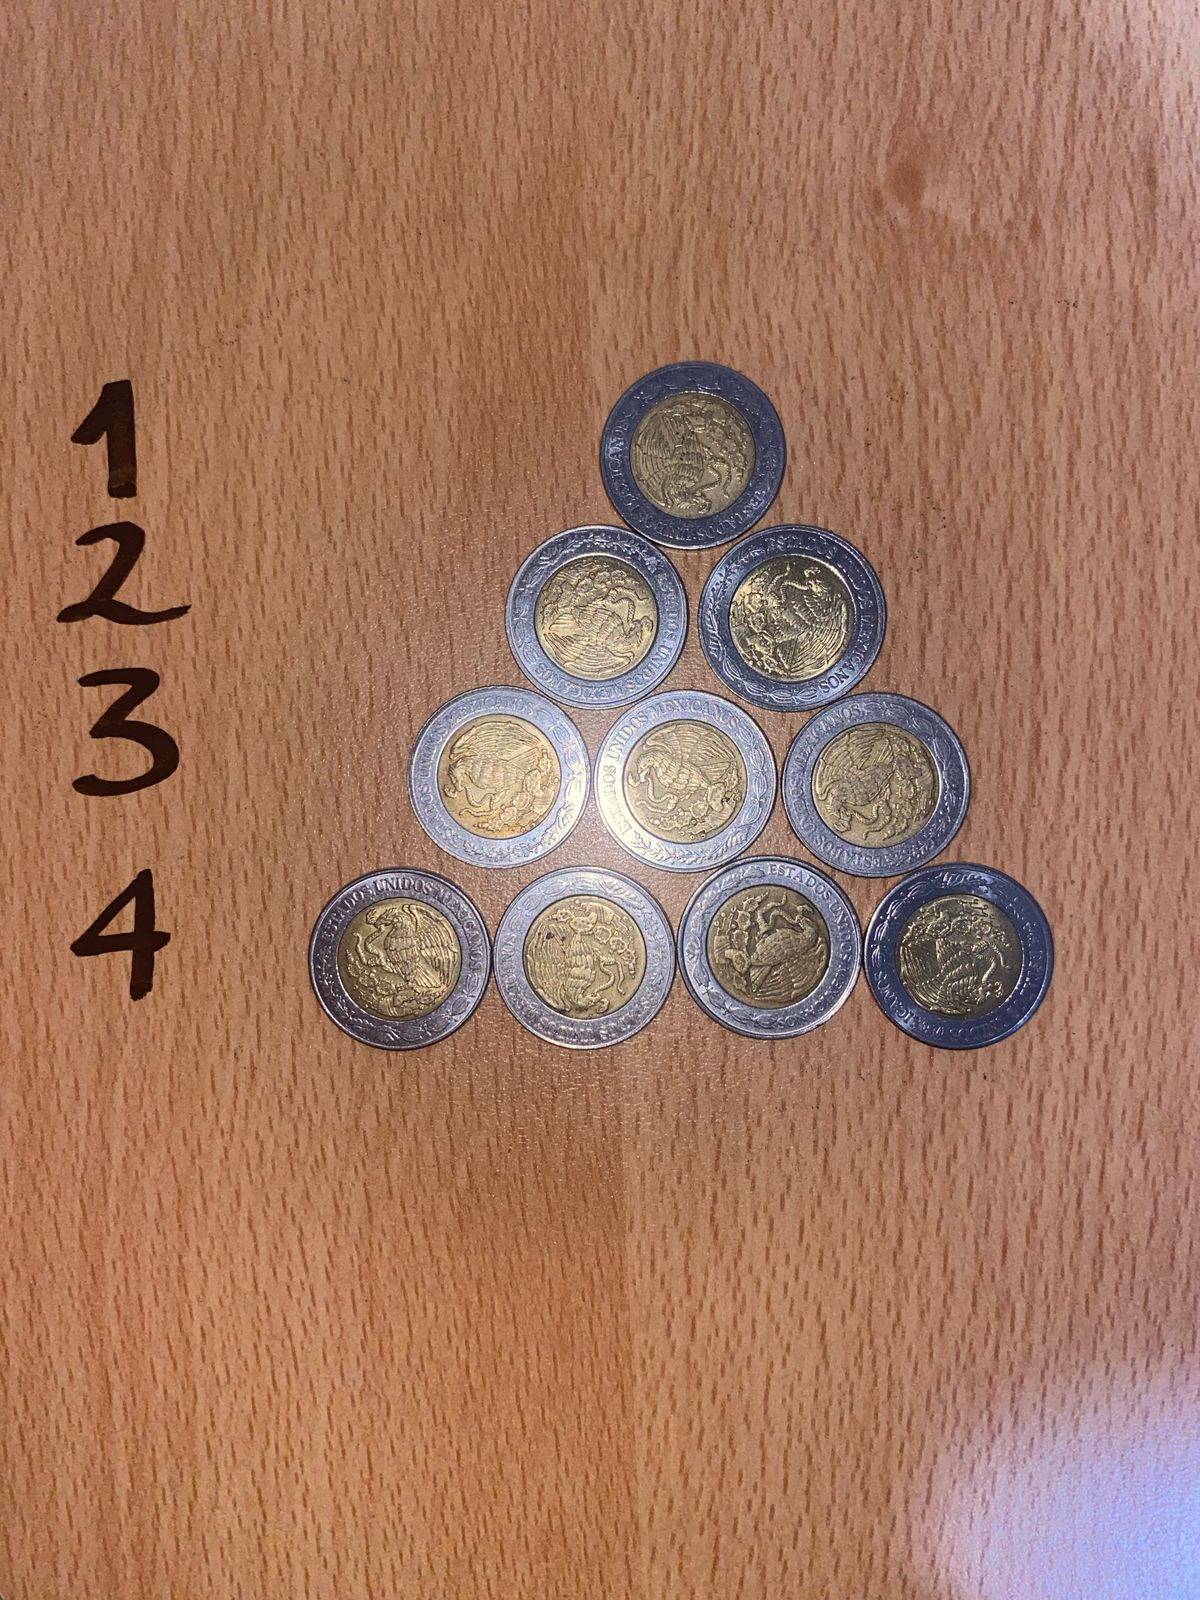
\includegraphics[scale=0.09]{clase3/FlechaEnum.jpeg}&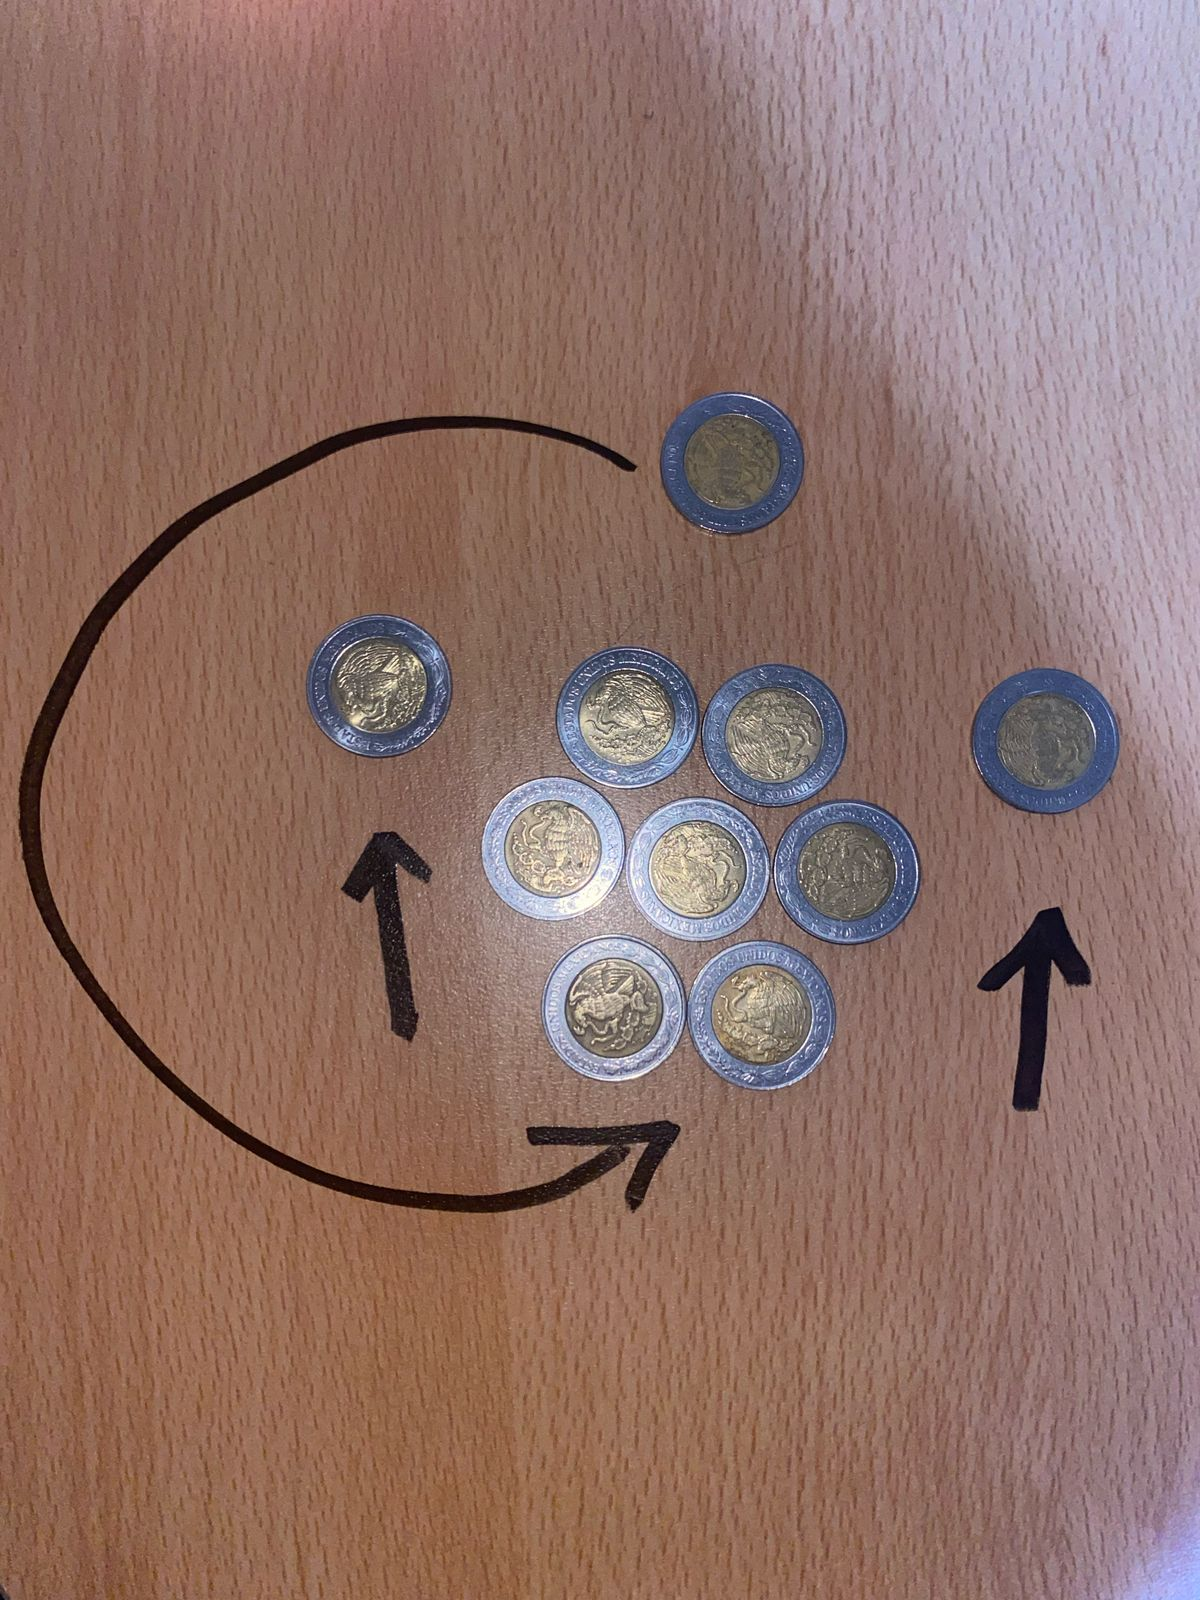
\includegraphics[scale=0.09]{clase3/base4punta1.jpeg}&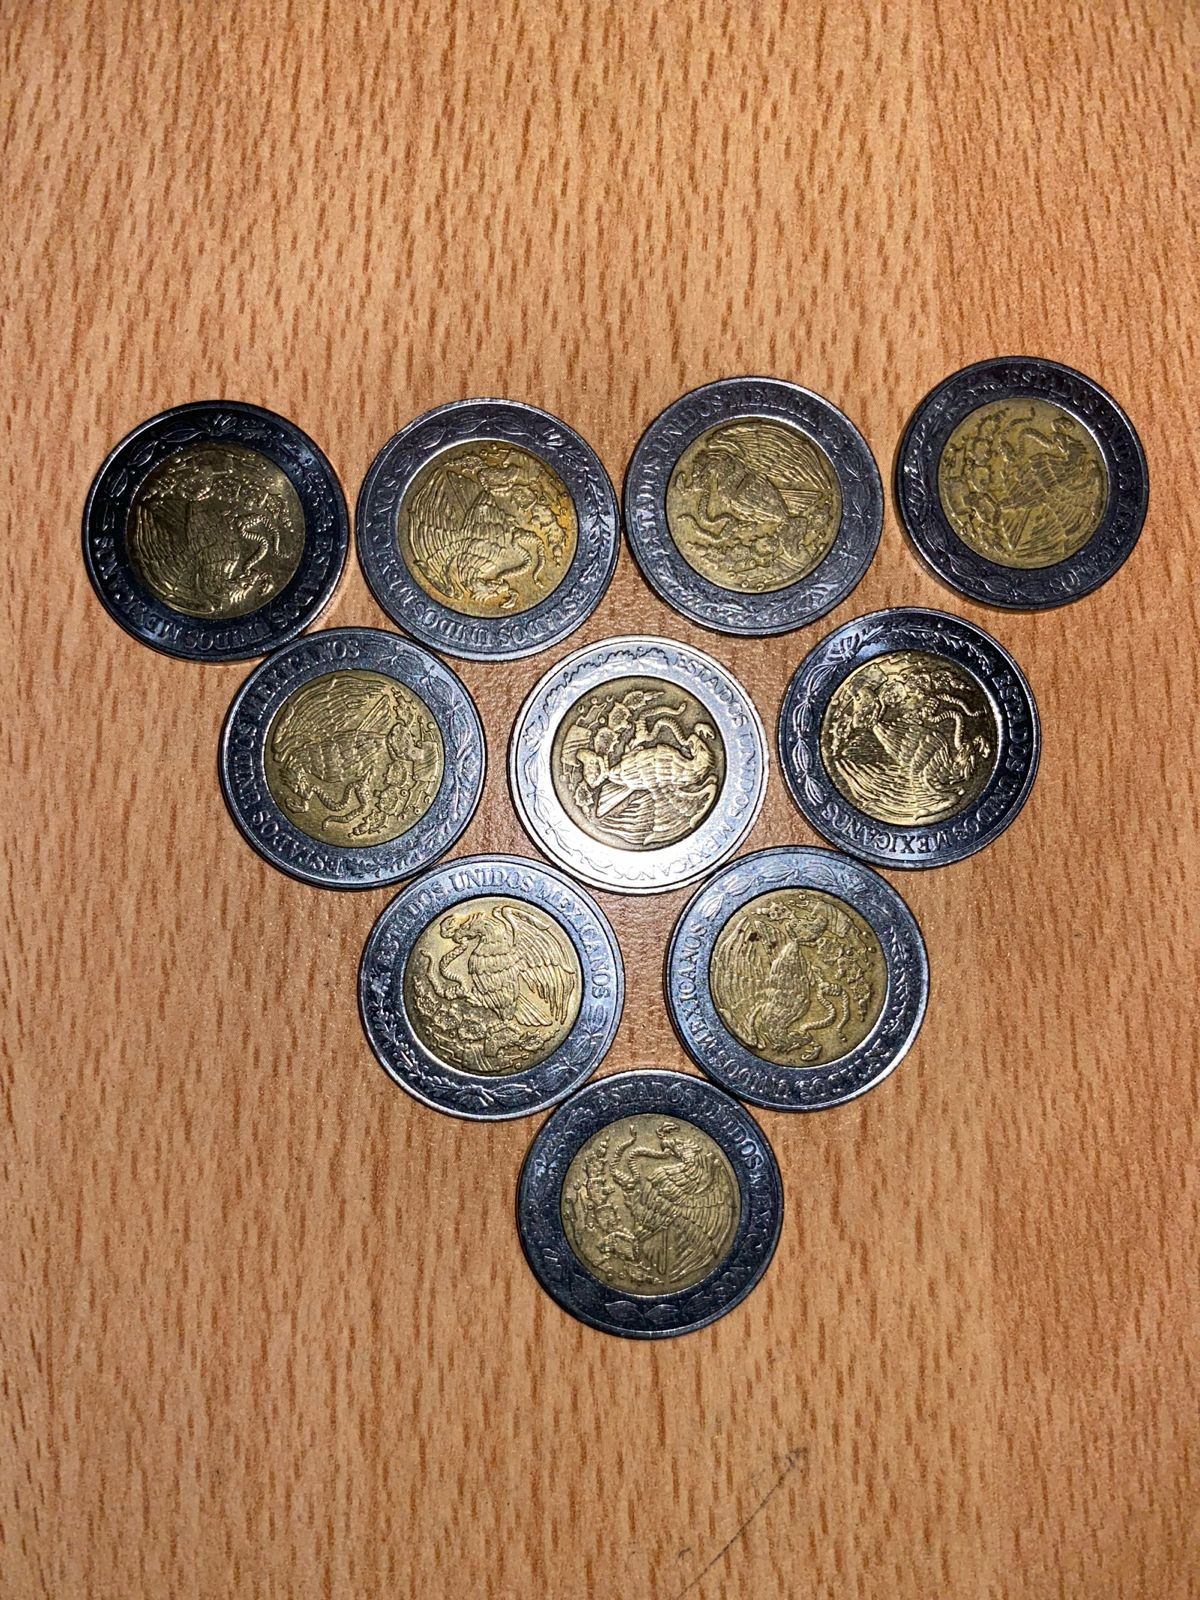
\includegraphics[scale=0.09]{clase3/FlechaInvertida.jpeg}
      \end{tabular}

   \end{center}   

   \textbf{SOLUCIÓN 2.} La segunda solución que encontramos fue ver la foto de las monedas, como un triángulo y mover únicamente los vértices, dado que las otras monedas en ningún momento se movían al poner la punta de flecha en cualquier dirección cumpliendo así la regla de sólo mover tres monedas a la vez.

   \begin{center}
      
      \begin{tabular}{c c c}
            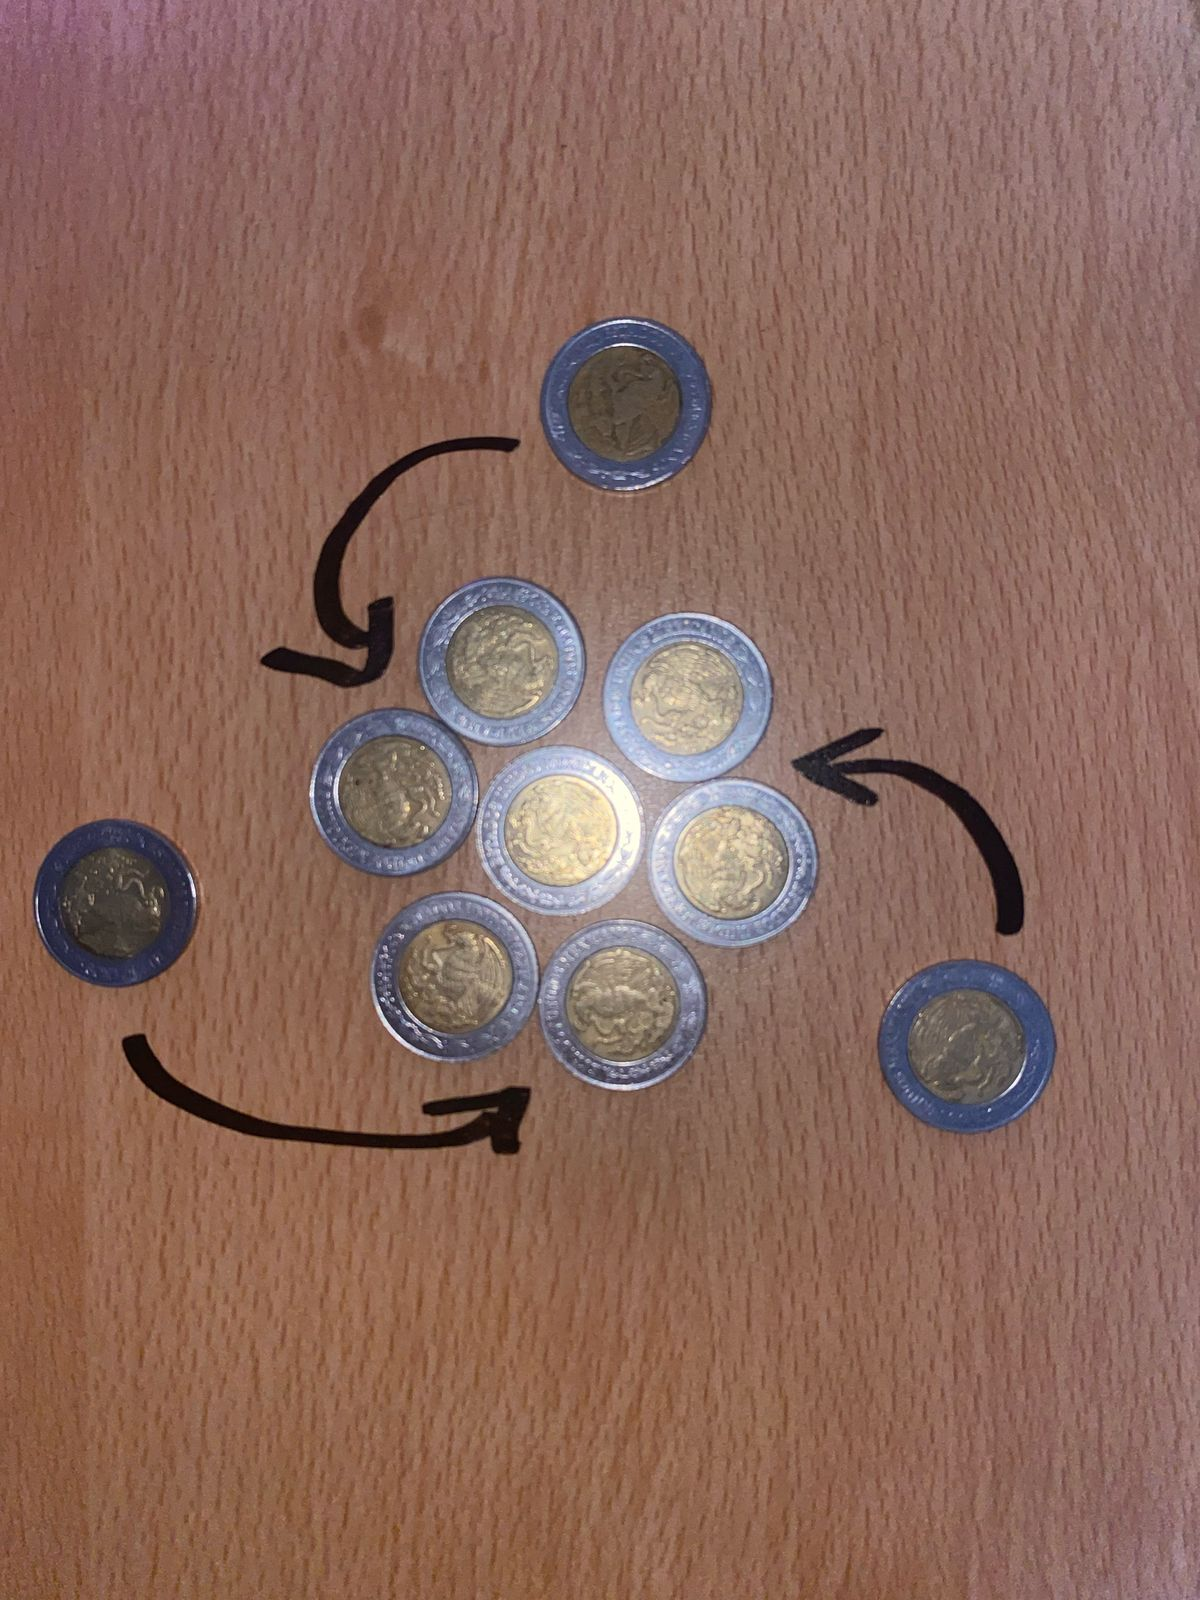
\includegraphics[scale=0.09]{clase3/rotacionVertices.jpeg}&&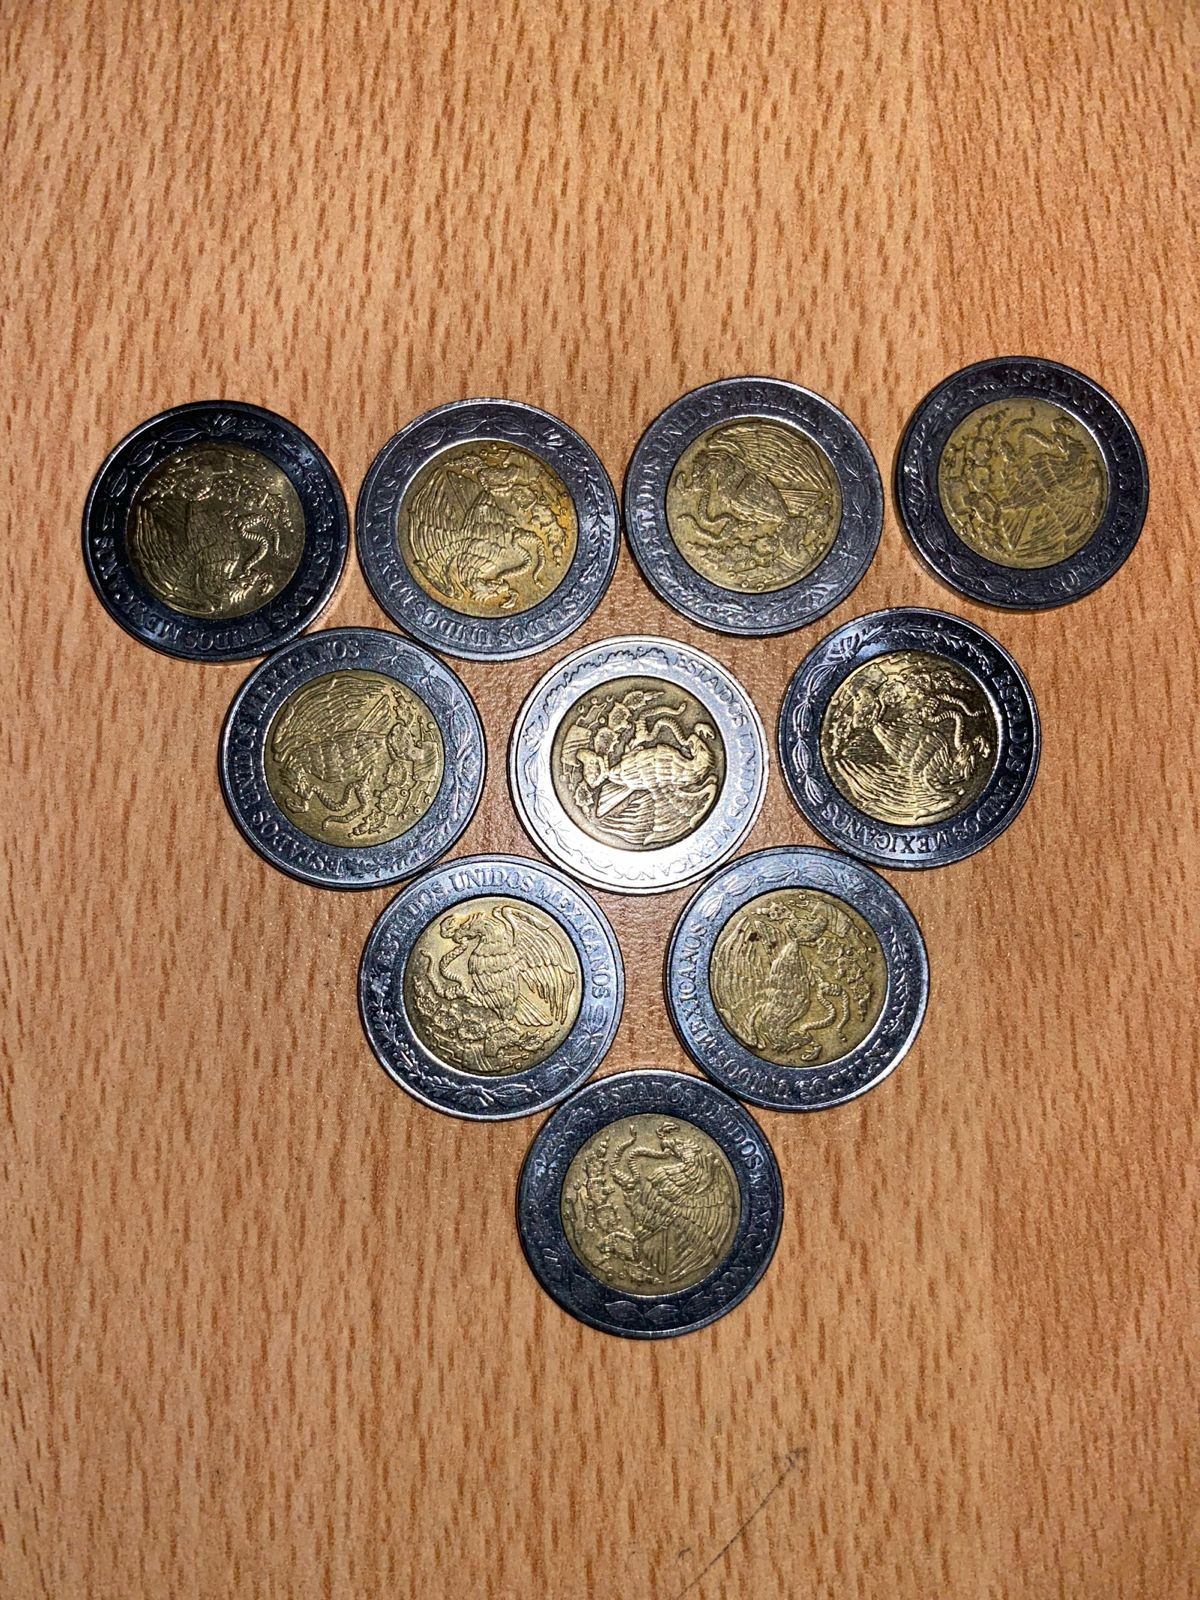
\includegraphics[scale=0.09]{clase3/FlechaInvertida.jpeg}
      \end{tabular}
      
   \end{center}   